\documentclass{article}
\usepackage{hyperref}
\usepackage[utf8]{inputenc}
\usepackage{graphicx}
\usepackage{ragged2e}
\usepackage{listings}
\usepackage{xcolor}
\usepackage{colortbl}
\usepackage{color}
\usepackage{array}
\usepackage{capt-of}
\usepackage{csvsimple}
\usepackage{definitions}
\lstset { %
    language=C,
    backgroundcolor=\color{black!5}, % set backgroundcolor
    basicstyle=\footnotesize,% basic font setting
}
\graphicspath{{img/}} 
\begin{document}
%titlepage
\makeatletter
\begin{titlepage}
\thispagestyle{empty}
\begin{center}
	\centering
	\vspace{1cm}
	{\scshape\Large PAR Laboratory Assignment\par}
	\vspace{0.75cm}
	{\Large Course 2018/19 (Fall semester)\par}
	\vspace{0.75cm}
	{\huge\bfseries Lab 4: Branch and bound with OpenMP: N-queens puzzle\par}
	\vspace{1cm}
	{\Large\itshape Pablo Vizcaino, Guillem Ramírez\par}
    \vspace{0.5cm}
    {\Large User: Par2206\par}
    \vfill
% Bottom of the page
	{\large \today\par}
\end{center}
\clearpage
\end{titlepage}

\clearpage
\tableofcontents
\clearpage 


%%%%%%INTRODUCTION%%%%%%%%%%%%%%%%%%%%%%%%%%%%%%%%%%%%%%%%%%%%%%%%%%%%%%%%%%%%%%%%%%%%%%%%%%%%%%%%%%%%%%%%
\section{Introduction}
\justify
In this laboratory assignment we are going to study and analyze 
the parallelization of Divide and Conquer algorithms using \textit{\omp},
specifically Mergesort.

\justify
We will be working with a  Multisort algorithm that combines a 
Divide and Conquer strategy (mergesort) with an iterative strategy (quicksort).

\justify
Multisort algorithm divides the vector in parts and when the divisions 
are small enough the quicksort algorithm is applied, named \textit{basicsort} in the code. 
Finally the sorted parts get merged into bigger sorted parts until we get the sorted vector.

\justify
In this laboratory assignment we are going to analyze, parallelize and evaluate this Divide and Conquer aproach using \textit{\omp} and \bsc performance analysis tools\footnote{\tools}. We are going to explore different strategies and pragmas to program the optimum version.
\clearpage
%%%%%%END OF INTRODUCTION%%%%%%%%%%%%%%%%%%%%%%%%%%%%%%%%%%%%%%%%%%%%%%%%%%%%%%%%%%%%%%%%%%%%%%%%%%%%%%%%%%%%%%%%

%%%%%%ANALYSIS WITH TAREADOR%%%%%%%%%%%%%%%%%%%%%%%%%%%%%%%%%%%%%%%%%%%%%%%%%%%%%%%%%%%%%%%%%%%%%%%%%%%%%%%%%%%%%%%%
\section{Task decomposition analysis using Tareador} \label{tasktareador}
\justify
In this section we are going to analyze the task decomposition for the
mergesort algorithm. We are going to use tareador to analyze dependencies
and consequently set up the parallelization strategies.
\justify
First of all we nedded to add Tareador instrumentation in order 
to get dependency graphs.
We added to the base code \texttt{tareador\_start\_task(task\_name)} and 
\texttt{tareador\_end\_task(task\_name)} clauses to the recursive calls
of
multisort:
\begin{lstlisting}
  tareador_start_task("multi1");
  multisort(n/4L, &data[0], &tmp[0]);
  tareador_end_task("multi1");
\end{lstlisting}
Also, we added them to mergesort recursive calls: 
\begin{lstlisting}
  tareador_start_task("merge1");
  merge(n, left, right, result, start, length/2);
  tareador_end_task("merge1");
\end{lstlisting}

\justify
Finally we compiled\footnote{make multisort-tareador} and runned\footnote{./run-tareador.sh multisort-tareador}
the modified version of the code obtaining the following graph.
\begin{figure}[h!]
    \centering
    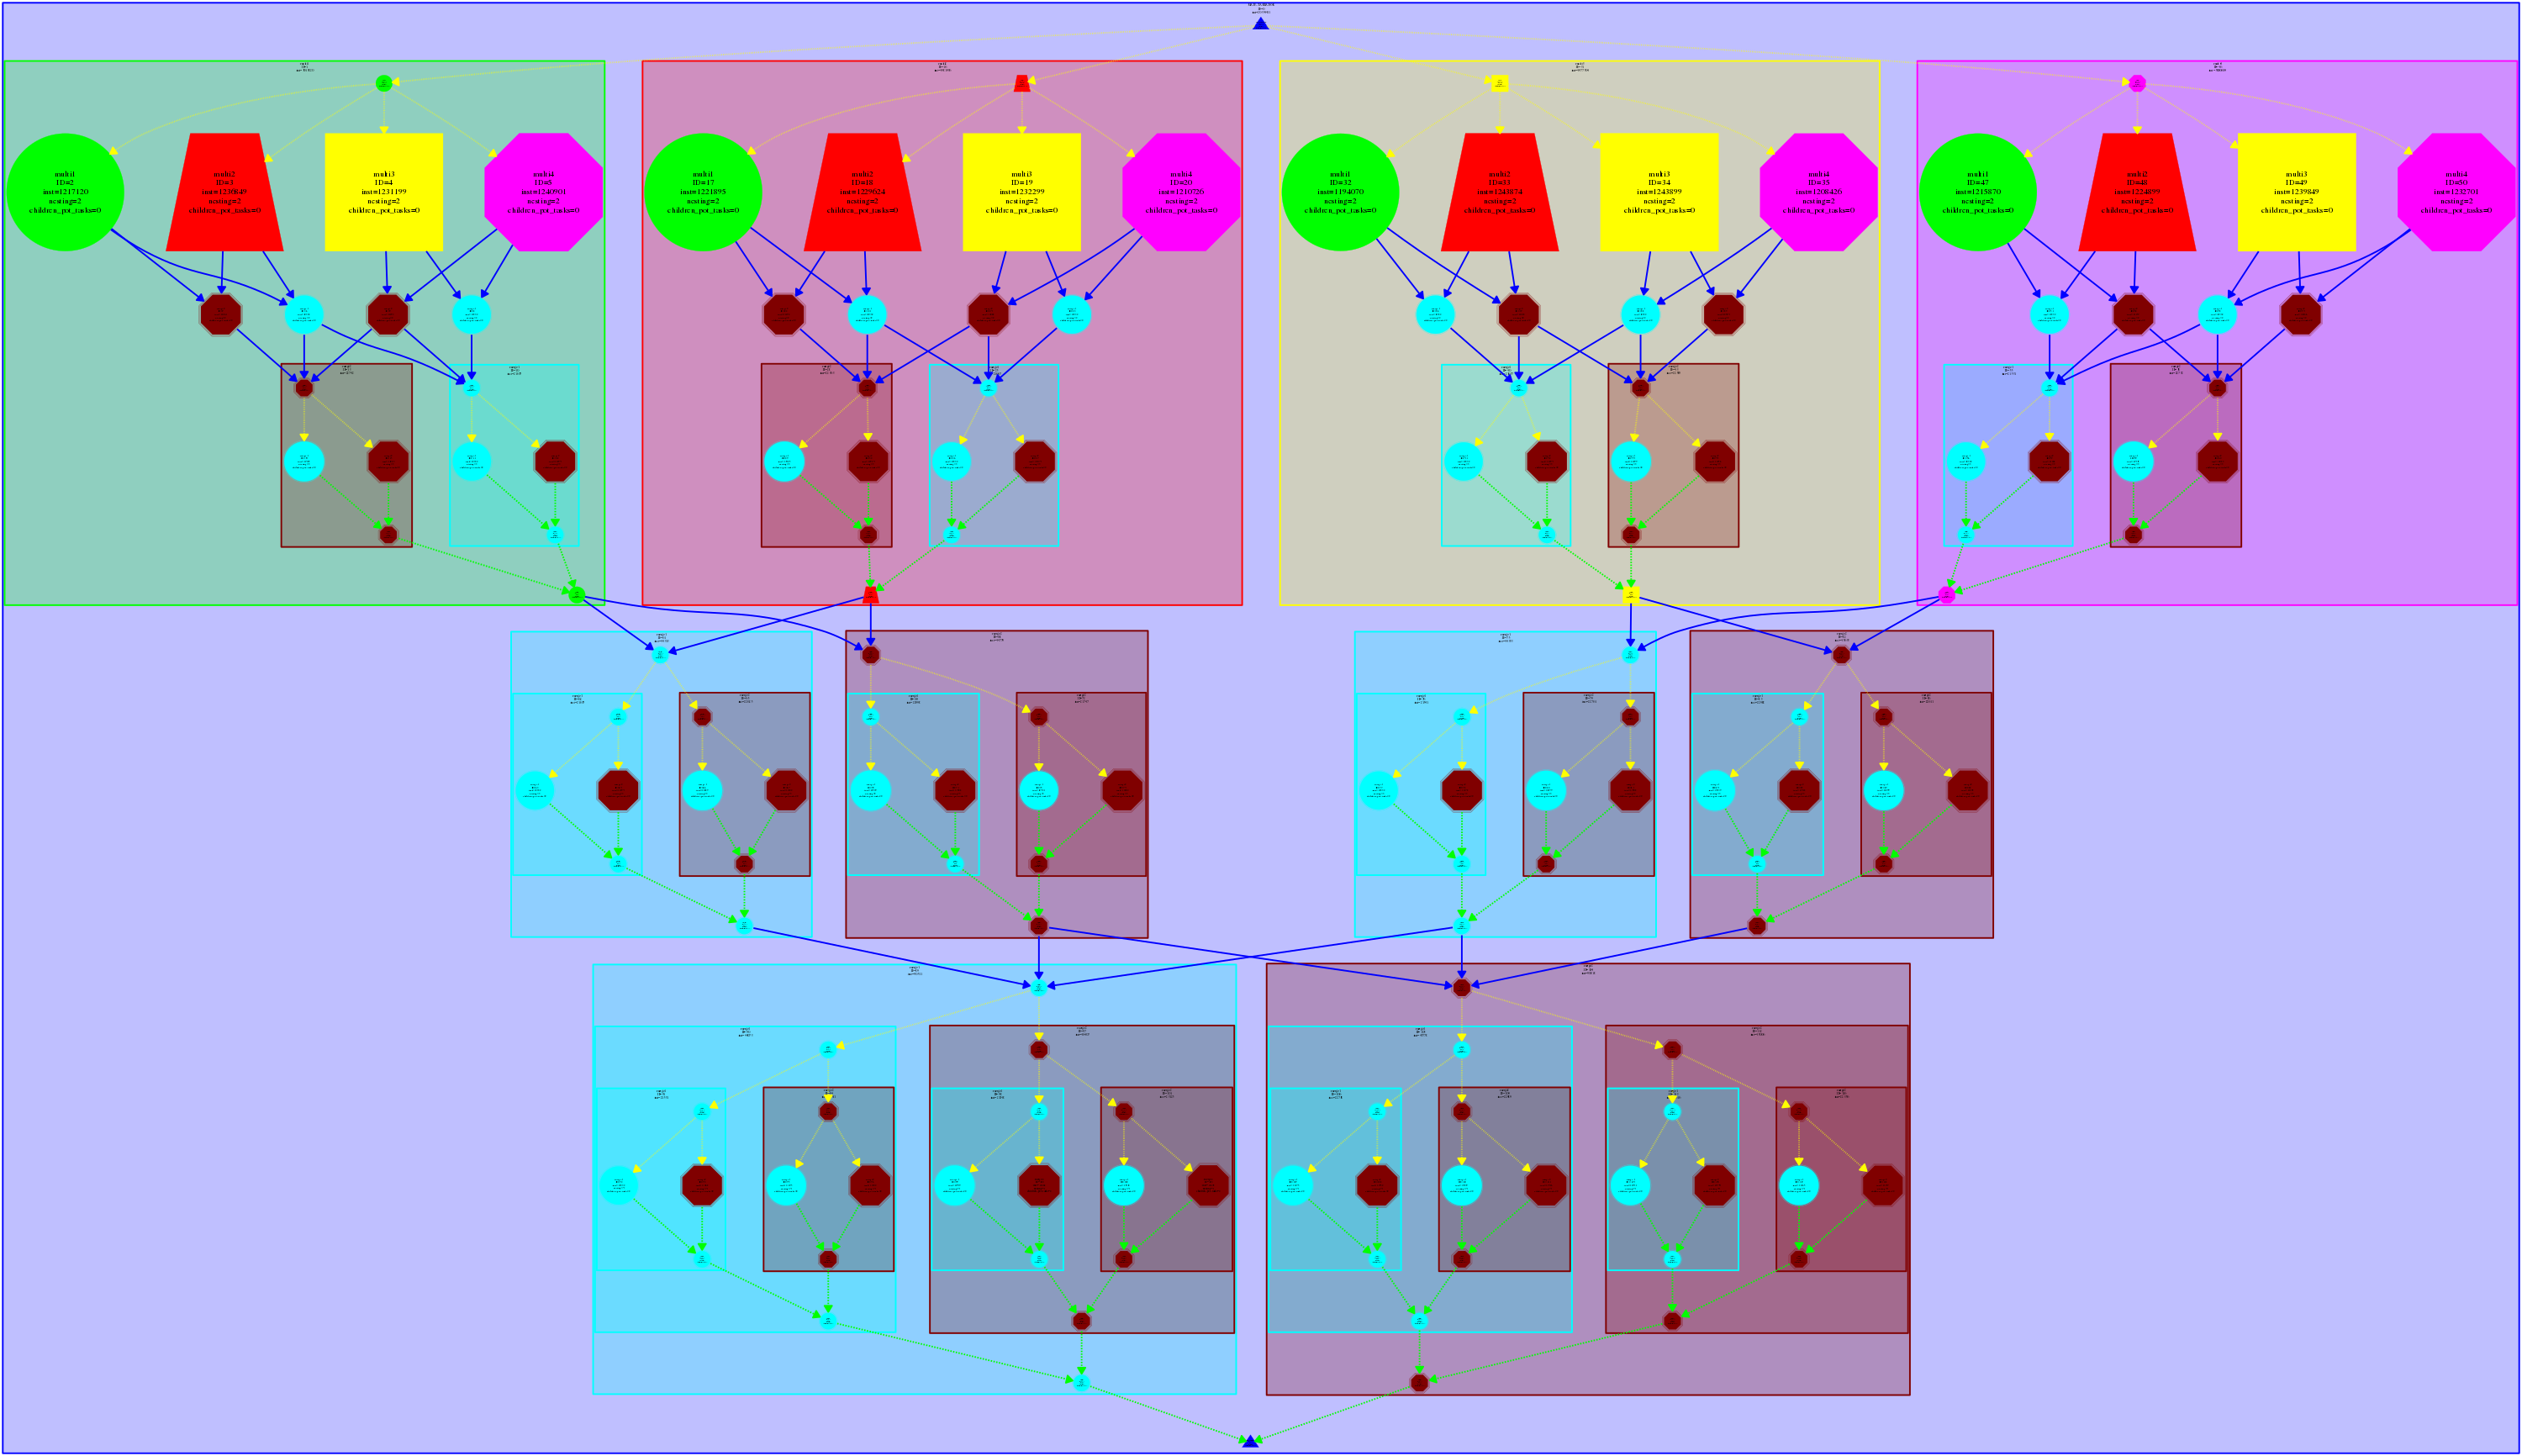
\includegraphics[width=0.99\textwidth]{tareador1.png}
    \caption{Tareador task decomposition graph}
    \label{fig:tareador}
\end{figure}
\justify
From the graph, we can observe that there are dependencies between tasks.
Specifically, each merge task has to wait to the two multisort tasks that are sorting the two parts that it needs to merge. Lastly, another merge has to wait the last merges in order to merge both of them.
\clearpage
\begin{figure}[!h]
\centering
\begin{minipage}[t]{.62\textwidth}
\centering
\vspace{0pt}
\justify
In order to evaluate its scallability we simulated its execution with 1,2,4,8,16,32 and 64 processors, gathered the execution time and calculated the respective speed-up from the version with 1 cpu.
\justify
In the table we can see that the speed-up is really close to the ideal case , because doubling the resources nearly doubles the speed-up. We can also observe that after 16 processors, adding more resources doesn't improve the performance. This is due to the size of the problem; we only divide the vector a finite amount of times, creating a finite amount of parallel tasks. Once we reach that limit, adding more resources doesn't increase the performance.
\end{minipage}\hfill
\begin{minipage}[t]{.35\textwidth}
\centering
\vspace{0pt}
\begin{tabular}{|l||l|l|}
\hline
\#cpu & t(s)  & s     \\ \hline
1     & 20.33 & 1     \\ \hline
2     & 10.17 & 1.99  \\ \hline
4     & 5.086 & 3.99  \\ \hline
8     & 2.55  & 7.97  \\ \hline
16    & 1.29  & 15.76 \\ \hline
32    & 1.29  & 15.76 \\ \hline
64    & 1.29  & 15.76 \\ \hline
\end{tabular}
\end{minipage}
\end{figure}

%%%%%%END OF ANALYSIS WITH TAREADOR%%%%%%%%%%%%%%%%%%%%%%%%%%%%%%%%%%%%%%%%%%%%%%%%%%%%%%%%%%%%%%%%%%%%%%%%%%%%%%%%%%%%%%%%

%%%%%%PARALLELIZATION STRATEGIES%%%%%%%%%%%%%%%%%%%%%%%%%%%%%%%%%%%%%%%%%%%%%%%%%%%%%%%%%%%%%%%%%%%%%%%%%%%%%%%%%%%%%%%%
\clearpage
\section{Parallelization strategies}
\justify
In this section we are going to compare two recursive parallelization strategies: leaf and tree. 
\subsection{Leaf strategy}
\justify
First we implemented the leaf strategy. To do so, we don't create tasks until
the code reaches the base case of the recursion. In the merge function we just have to add a task creation in the base case.
\begin{lstlisting}
void merge(long n, T left[n], T right[n], T result[n*2], 
           long start, long length) {
        if (length < MIN_MERGE_SIZE*2L) {
                // Base case
                #pragma omp task 
                basicmerge(n, left, right, result, start, length);
        } else {
                // Recursive decomposition
                merge(n, left, right, result, start, length/2);
                merge(n, left, right, result, start + length/2, 
                length/2);
        }
}
\end{lstlisting}
\justify
In the multisort routine we added a task creation pragma in the base case and also implemented a task synchronization mechanism using \texttt{\#pragma omp taskwait} in order to respect data dependencies. 
\begin{lstlisting}
void multisort(long n, T data[n], T tmp[n]) {
        if (n >= MIN_SORT_SIZE*4L) {
                // Recursive decomposition
                multisort(n/4L, &data[0], &tmp[0]);
                multisort(n/4L, &data[n/4L], &tmp[n/4L]);
                multisort(n/4L, &data[n/2L], &tmp[n/2L]);
                multisort(n/4L, &data[3L*n/4L], &tmp[3L*n/4L]);
                #pragma omp taskwait
                merge(n/4L, &data[0], &data[n/4L], &tmp[0], 0, 
                      n/2L);
                merge(n/4L, &data[n/2L], &data[3L*n/4L], &tmp[n/2L], 
                      0, n/2L);
                #pragma omp taskwait
                merge(n/2L, &tmp[0], &tmp[n/2L], &data[0], 0, n);
        } else {
                // Base case
                #pragma omp task 
                basicsort(n, data);

        }
}
\end{lstlisting}
\clearpage
We can observe this strategy's impact in the paraver timeline. It can be seen that only the first thread is creating tasks and synchronizing them. The other threads are only executing tasks, which are the base cases.
\begin{figure}[!h]
    \centering
    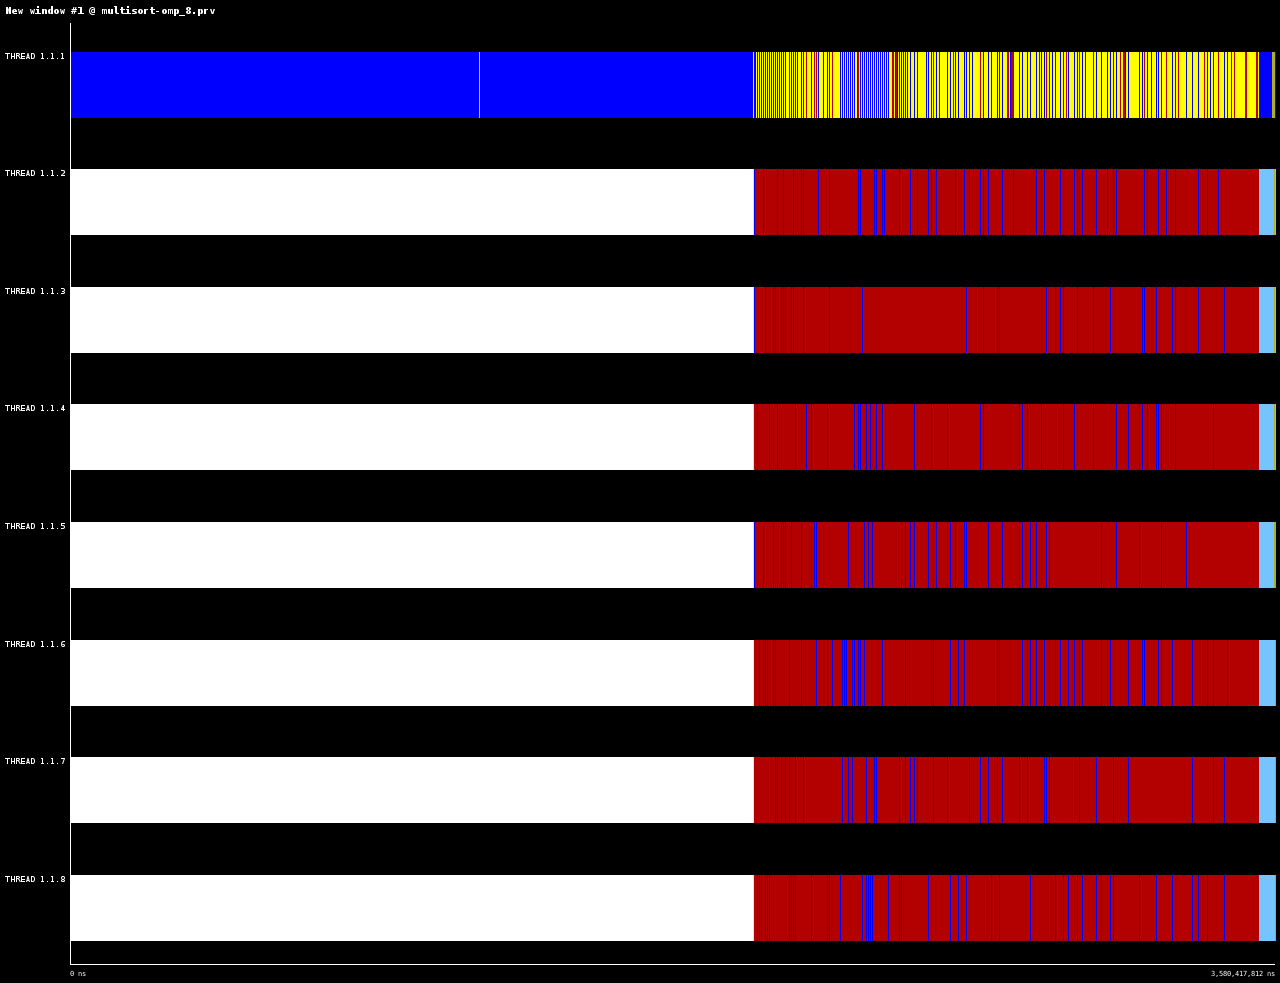
\includegraphics[width=0.65\textwidth]{paraver_noCFG_leafNC.png}
    \caption{Paraver timeline for leaf strategy}
    \label{fig:tareador}
\end{figure}
\justify
The number of task creations (bursts) that we obtained is 11264 and the execution time of this parallelizable part is 1.525s. This will be usefull to compare it with the next strategy.
\justify
In order to analyze the strategy's performance, we obtained the strong speed-up plots.
\begin{figure}[!h]
    \centering
    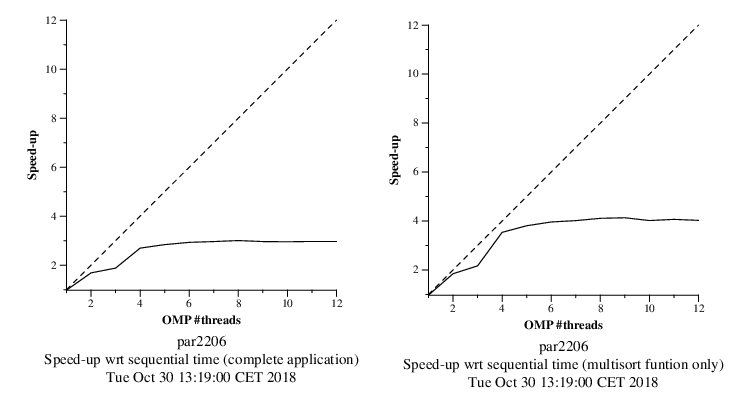
\includegraphics[width=0.78\textwidth]{strongLeafNC.png}
    \caption{Strong speed-up plots for leaf strategy}
    \label{fig:tareador}
\end{figure}
\justify
We can observe that after 4 threads the speed is nearly constant, making it far from ideal. 
%%%%%%END PARALLELIZATION STRATEGIES%%%%%%%%%%%%%%%%%%%%%%%%%%%%%%%%%%%%%%%%%%%%%%%%%%%%%%%%%%%%%%%%%%%%%%%%%%%%%%%%%%%%%%%%
\subsection{Tree strategy} \label{treeST}
\justify
The second strategy that we implemented was the tree strategy. To do so, we create the tasks in each recursion call. In the merge function we added a \texttt{\#pragma omp task} before each recursion call and a \texttt{\#pragma omp taskwait} at the end for synchronization.
\begin{lstlisting}
void merge(long n, T left[n], T right[n], T result[n*2],
           long start, long length) {
        if (length < MIN_MERGE_SIZE*2L) {
                // Base case
                basicmerge(n, left, right, result, start, length);
        } else {
                // Recursive decomposition
                #pragma omp task
                 merge(n, left, right, result, start, length/2);
                #pragma omp task
                merge(n, left, right, result, start + length/2,
                      length/2);
                #pragma omp taskwait
        }
}
\end{lstlisting}
\justify
In the multisort function we applied the same logic. We added a \texttt{\#pragma omp task} before each recursion call and then added the needed task synchronization pragmas guided by the dependencies we found at section \ref{tasktareador}.
\begin{lstlisting}
void multisort(long n, T data[n], T tmp[n]) {
        if (n >= MIN_SORT_SIZE*4L) {
                // Recursive decomposition
                #pragma omp task
                multisort(n/4L, &data[0], &tmp[0]);
                #pragma omp task
                multisort(n/4L, &data[n/4L], &tmp[n/4L]);
                #pragma omp tas
                multisort(n/4L, &data[n/2L], &tmp[n/2L]);
                #pragma omp task
                multisort(n/4L, &data[3L*n/4L], &tmp[3L*n/4L]);
                #pragma omp taskwait

                #pragma omp task
                merge(n/4L, &data[0], &data[n/4L], &tmp[0],0,n/2L);
                #pragma omp task
                merge(n/4L, &data[n/2L], &data[3L*n/4L], &tmp[n/2L],
                      0, n/2L);
                #pragma omp taskwait
                
                #pragma omp task
                merge(n/2L, &tmp[0], &tmp[n/2L], &data[0], 0, n);
                #pragma omp taskwait
        } else {
                // Base case
                basicsort(n, data);
        }
}       
\end{lstlisting}
\justify
When looking at the paraver timeline of this strategy, we can see that unlike the leaf strategy all threads are creating and synchronizing tasks.
\begin{figure}[!h]
    \centering
    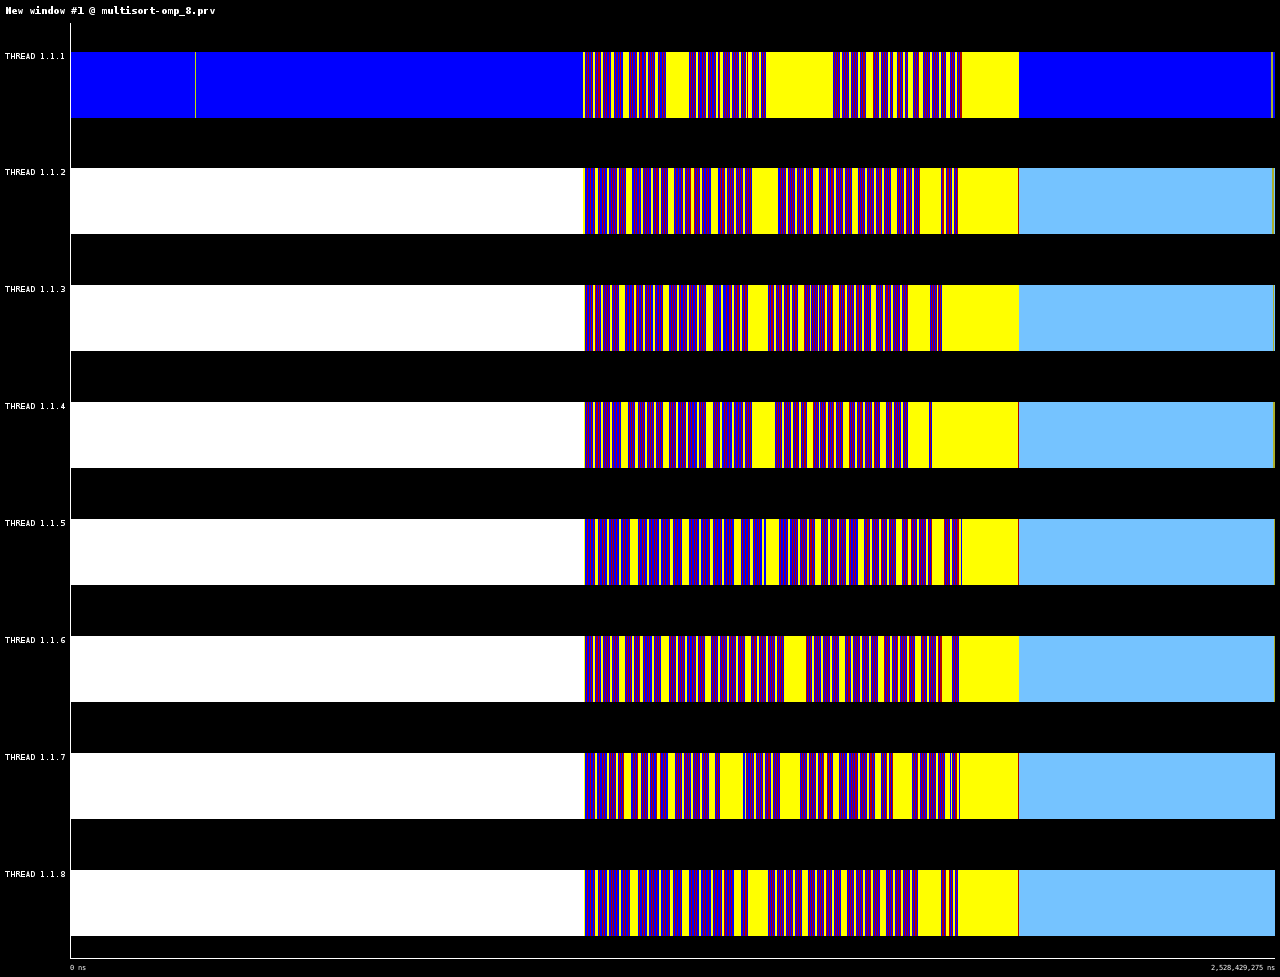
\includegraphics[width=0.65\textwidth]{paraver_noCFG_treeNC.png}
    \caption{Paraver timeline for tree strategy}
    \label{fig:}
\end{figure}

\justify

Another metric when comparing it to the leaf strategy is the number of task creations of the new strategy. In this case, we obtained 20821 burst, 78\% more than the leaf version. This makes sense considering that the tree strategy creates tasks as it travels the recursive tree.
\justify
The most distinctive metric that helped us choose the tree strategy as the better one (in this given problem) is the execution time of the parallelizable part. The time we obtained is 0.88s, a speed-up of 1.73 when comparing it to the leaf strategy.
\clearpage
\justify
For comparing both strategies we also obtained the strong scalability plots of the tree version.
\begin{figure}[!h]
    \centering
    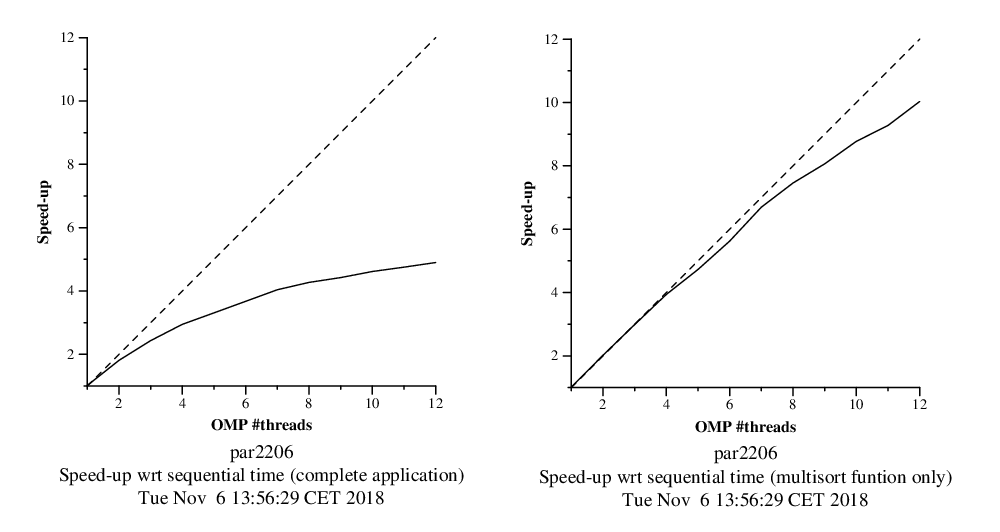
\includegraphics[width=0.99\textwidth]{treeStrongNC.png}
    \caption{Strong scalability plot for tree strategy}
    \label{fig:}
\end{figure}
\justify
From the strong scalability plots we can observe that this strategy is much better than the leaf one, as it gets much closer to the ideal speed-up. 


%%%%%%%%%%%%%%%%%%%%%%%%%%% IMPROVING TREE STRATEGY %%%%%%%%%%%%%%%%%%%%%%%%%%%%%%%%

\clearpage
\section{Improving tree strategy}
\justify
As wee seen in the section \ref{treeST}, the tree strategy went much better on solving the problem, as its execution time nearly halved. In this section we are going to implement some improvements with the goal to get a smaller execution time, reducing overheads.

\subsection{Cut off}
\justify
A problem that the original tree version has is that there is no cutoff mechanism implemented. So in big problem sizes we can find out that we have overheads; the program would create exponentially too many tasks as it goes deeper in recursion.

\justify
To control the creation of tasks, we need to implement a cut off control mechanism. This is done adding \texttt{\#task final(d>=CUTOFF) mergeable} and modifying our functions to have a depth counter. What the \texttt{final} clause does is stopping the parallelization of the program once the condition evaluated is true. When that happens, the threads that reach the pragma will switch to the execution of the new task instead of running it simultaneously, effectively stopping the parallelization.
One important note in our implementation is that the merge function doesnt get a new value of depth when it's called from the multisort function; even tho it does its own recursion.
\newline
\begin{lstlisting}
void merge(long n, T left[n], T right[n], T result[n*2], long start,
           long length,int d) {
        if (length < MIN_MERGE_SIZE*2L) {
                // Base casea
                basicmerge(n, left, right, result, start, length);
        } else {
                // Recursive decomposition
                #pragma omp task final(d>=CUTOFF) mergeable
                 merge(n, left, right, result, start, length/2,d+1);
                #pragma omp task final(d>=CUTOFF) mergeable
                merge(n, left, right, result, start + length/2,
                      length/2,d+1);
                #pragma omp taskwait
        }
}

void multisort(long n, T data[n], T tmp[n], int d) {
        if (n >= MIN_SORT_SIZE*4L) {
                // Recursive decomposition
                #pragma omp task final(d>=CUTOFF) mergeable
                multisort(n/4L, &data[0], &tmp[0],d+1);
                #pragma omp task final(d>=CUTOFF) mergeable
                multisort(n/4L, &data[n/4L], &tmp[n/4L],d+1);
                #pragma omp task final(d>=CUTOFF) mergeable
                multisort(n/4L, &data[n/2L], &tmp[n/2L],d+1);
                #pragma omp task final(d>=CUTOFF) mergeable
                multisort(n/4L, &data[3L*n/4L], &tmp[3L*n/4L],d+1);
                #pragma omp taskwait

                #pragma omp task final(d>=CUTOFF) mergeable
                merge(n/4L, &data[0], &data[n/4L], &tmp[0], 0, n/2L
                      ,d+1);

                #pragma omp task final(d>=CUTOFF) mergeable
                merge(n/4L, &data[n/2L], &data[3L*n/4L], &tmp[n/2L]
                      , 0, n/2L, d+1);
                #pragma omp taskwait

                #pragma omp task final(d>=CUTOFF) mergeable
                merge(n/2L, &tmp[0], &tmp[n/2L], &data[0], 0, n,
                      d+1);
                #pragma omp taskwait
        } else {
                // Base case
                basicsort(n, data);

        }
}
\end{lstlisting}
\justify
Once we have this mechanism implemented, we need to evaluate the optimum value of the \textit{CUTOFF} variable. To do so, we used the script that was given to us that tries different values and calculates the execution time with that \textit{cutoff}. We made a small modification, making the script try some more and bigger values of the cutoff to really see the optimal one.

\begin{figure}[!h]
    \centering
    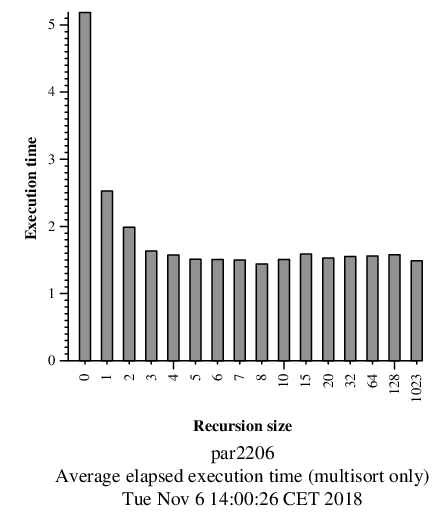
\includegraphics[width=0.5\textwidth]{cutoffEvaluation.png}
    \caption{Execution time with different values of cutoff }
    \label{fig:tareador}
\end{figure}

\justify
As it can be seen in the figure, the optimal \textit{cutoff} value is 8.
\clearpage
The next step was to evaluate this new version with this value. In order to do that, the first thing we did was to obtain the execution time. This version spent 0.879s on the parallelizable part, not really improving the previous time by any significant amount. This is due to the small number of recursive calls the program actually does. If the problem size was larger, the overheads would be much bigger and this mechanic would be much more effective.
\justify
In order to see some differences with the previous version, first we will look at the task profile table inside paraver. The numbers are the bursts.


\begin{table}[!h]
\begin{tabular}{l|ll|ll|}
\cline{2-5}
                                   & No cutoff                         &          & Cutoff                            &          \\ \hline
\multicolumn{1}{|l|}{\#thread}     & \multicolumn{1}{l|}{instantiated} & executed & \multicolumn{1}{l|}{instantiated} & executed \\ \hline
\multicolumn{1}{|l|}{THREAD 1.1.1} & \multicolumn{1}{l|}{5924}         & 3022     & \multicolumn{1}{l|}{3244}         & 3259     \\ \hline
\multicolumn{1}{|l|}{THREAD 1.1.2} & \multicolumn{1}{l|}{4851}         & 2496     & \multicolumn{1}{l|}{2568}         & 2573     \\ \hline
\multicolumn{1}{|l|}{THREAD 1.1.3} & \multicolumn{1}{l|}{5467}         & 2496     & \multicolumn{1}{l|}{2428}         & 2436     \\ \hline
\multicolumn{1}{|l|}{THREAD 1.1.4} & \multicolumn{1}{l|}{5615}         & 2868     & \multicolumn{1}{l|}{3096}         & 3101     \\ \hline
\multicolumn{1}{|l|}{THREAD 1.1.5} & \multicolumn{1}{l|}{4071}         & 2105     & \multicolumn{1}{l|}{2449}         & 2441     \\ \hline
\multicolumn{1}{|l|}{THREAD 1.1.6} & \multicolumn{1}{l|}{4770}         & 2454     & \multicolumn{1}{l|}{2391}         & 2391     \\ \hline
\multicolumn{1}{|l|}{THREAD 1.1.7} & \multicolumn{1}{l|}{5118}         & 2622     & \multicolumn{1}{l|}{2499}         & 2477     \\ \hline
\multicolumn{1}{|l|}{THREAD 1.1.8} & \multicolumn{1}{l|}{4799}         & 2454     & \multicolumn{1}{l|}{2146}         & 2143     \\ \hline
\end{tabular}
\end{table}

\justify
The new version spends a bigger percentatge of time executing than instantiating tasks when compared to the one without cutoff.
\justify
As usual, another graph that is useful when evaluating the performance of a parallel program is the strong scalability plot.

\begin{figure}[!h]
    \centering
    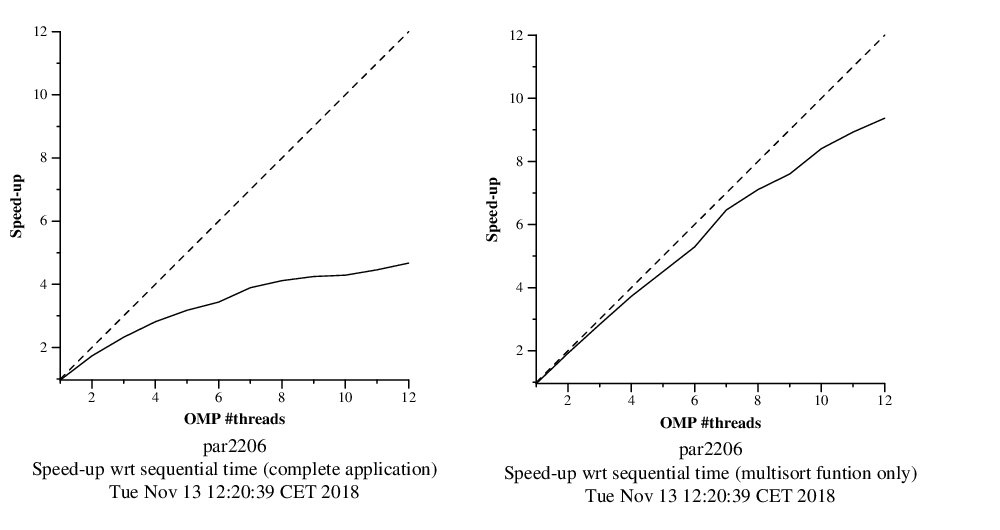
\includegraphics[width=0.9\textwidth]{treeStrongC.png}
    \caption{Execution time with different values of cutoff }
    \label{fig:tareador}
\end{figure}
\justify

This figure is very similar to its counterpart in the tree version without cutoff, because as we mentioned before the problem size isn't larger enough to create a big difference.

\justify
\subsection{Depend}
Another problem that can happen when parallelizing programs with dependences is that synchronization can be too strict. The pragmas that we used before wait until all other tasks of its level are finished before passing the barrier and executing new tasks, even if some of this new tasks don't depend on all the tasks that need to finish before passing the \textit{taskwait}.
\justify
To remove some of the \texttt{\#pragma omp taskwait} we can implement the task synchronization mechanism with \texttt{depend} \omp clauses. This clauses lets the programmer choose what work needs to be done before creating a specific task and what part of the work does it produces for other tasks to consume. 
\justify
In our problem, we identified specified which quarter of the vector does each multisort recursive call produce and which half does the merge calls use. Inside the merge function there's no dependence between each pair of calls, so we did not add the depend clause.


\begin{lstlisting}
void merge(long n, T left[n], T right[n], T result[n*2], long start
           ,long length,int d) {
        if (length < MIN_MERGE_SIZE*2L) {
                // Base casea
                basicmerge(n, left, right, result, start, length);
        } else {
                // Recursive decomposition
                #pragma omp task final(d>=CUTOFF) mergeable
                 merge(n, left, right, result, start, length/2,d+1);
                #pragma omp task final(d>=CUTOFF) mergeable
                merge(n, left, right, result, start + length/2
                      length/2,d+1);
                #pragma omp taskwait
        }
}

void multisort(long n, T data[n], T tmp[n], int d) {
        if (n >= MIN_SORT_SIZE*4L) {
                // Recursive decomposition
                #pragma omp task depend(out:data[0]) 
                          final(d>=CUTOFF) mergeable
                multisort(n/4L, &data[0], &tmp[0],d+1);
                #pragma omp task depend(out:data[n/4L]) 
                             final(d>=CUTOFF) mergeable
                multisort(n/4L, &data[n/4L], &tmp[n/4L],d+1);
                #pragma omp task depend(out:data[n/2L])
                             final(d>=CUTOFF) mergeable
                multisort(n/4L, &data[n/2L], &tmp[n/2L],d+1);
                #pragma omp task depend(out:data[3L*n/4L]) 
                                final(d>=CUTOFF) mergeable
                multisort(n/4L, &data[3L*n/4L], &tmp[3L*n/4L],d+1);
                
                #pragma omp task depend(in:data[0], data[n/4L])
                    depend(out: tmp[0]) final(d>=CUTOFF) mergeable
                merge(n/4L, &data[0], &data[n/4L], &tmp[0], 0, n/2L
                      , d+1);
                #pragma omp task depend(in:data[n/2L],
                   data[3L*n/4L]) depend(out: tmp[n/2L])
                   final(d>=CUTOFF) mergeable
                merge(n/4L, &data[n/2L], &data[3L*n/4L], &tmp[n/2L]
                      , 0, n/2L, d+1);
                #pragma omp task depend(in:tmp[0], tmp[n/2L])
                                   final(d>=CUTOFF) mergeable
                merge(n/2L, &tmp[0], &tmp[n/2L], &data[0], 0, n
                      ,d+1);
                #pragma omp taskwait
        } else {
                // Base case
                basicsort(n, data);

        }
}
\end{lstlisting}

\justify
To evaluate the improved version with the new definition of dependences, first we obtained the execution time of the parallelizable part and we got 0.87s, again a really small improvement. This is due to the fact that all recursive calls lasts nearly the same amount of time, so they most likely end together. The new tasks that are waiting for specific tasks and dependences to end (with the \textit{depend} clauses) would benefit from this new implementation if the task that they are waiting ended before the other ones. If they end at the same time, the result is the same as waiting all of them (as we did with the \textit{taskwait} clause).
\justify
Nonetheless, we also obtained the strong scalability plot and confirmed that the difference with the previous tree versions is minimal.

\begin{figure}[!h]
    \centering
    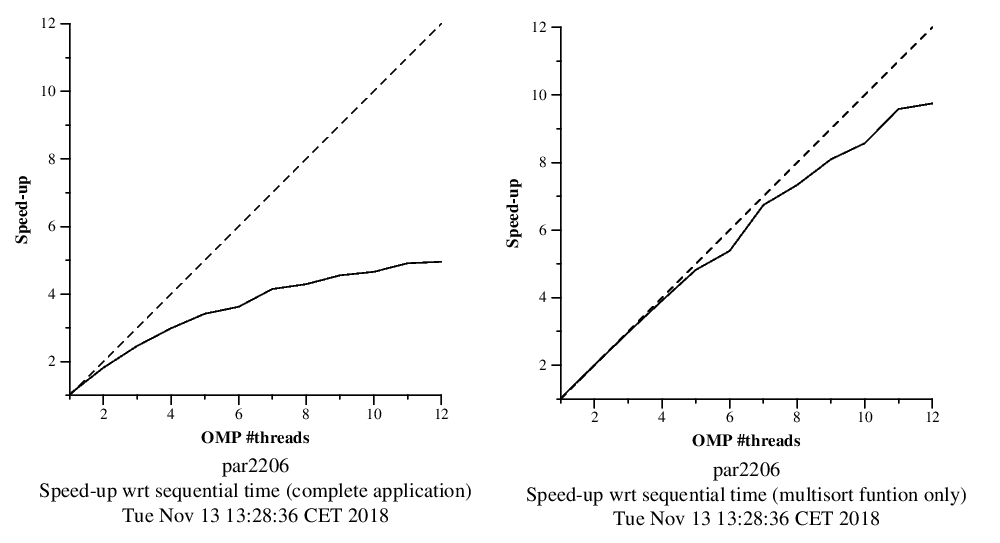
\includegraphics[width=0.9\textwidth]{treeCDepend.png}
    \caption{Speedup plots for depend version }
    \label{fig:tareador}
\end{figure}

\clearpage
\section{Conclusions}
\justify

In this laboratory assignment we consolidated the knowledge of the difference between leaf and tree parallelization strategies, and observed that in this kind of problems and with enough resources, the tree one is usually the best option. 
\justify
Another important thing that we learned to implement, even if it didn't have a big impact on our problem, is the cut-off mechanism. As we commented, it would have a much more important role if the problem size was bigger and we couldnt afford the overhead of creating too many tasks.
\justify
Lastly, we also learned to implement the \textit{depend} clause and most importantly to identify the exact dependences of each task in order to minimize the serialization of the program that implies using synchronization. The improvement wasn't big in our case, but we understood that it can greatly improve the execution time of another programs.

\end{document}
